\onehalfspacing

\chapter{Liquid-liquid phase separation for binary fluids}
\label{chap:Chapter_2}

The spontaneous segregation of a system into multiple phases of different composition is commonly called as Phase separation.
A frequent example of this phenomena is the formation of spherical oil droplets from water.
As we are primarily interested in modelling the dynamics of droplets which have been phase separated from a dilute phase, we will systematically build up the theory of phase separation.

In this chapter, we will start by deriving the basic thermodynamic principles governing Liquid-liquid phase separation for an incompressible binary fluid system, and we will discuss the nature and dynamics of various phases the system forms. 
First, we will restrict ourselves to passive phase separation.
We will later include the effects of chemical reactions, which are ubiquitous inside the biological cell, on the physics of phase separation.
We then focus on the situation where droplets are formed as a result of phase separation from the dilute phase and arrive at dynamical equations for describing such droplets and the dilute phase itself. 

\section{Thermodynamics of binary mixtures}
We consider an incompressible binary fluid system, consisting of two fluids $A,~B$.
We use the lattice description from classical thermodynamics and statistical mechanics to arrive at the total free energy of such a system; see Refs. \cite{balian2007microphysics1,balian2007microphysics2} as following.
On a lattice with $M$ lattice sites, consider that we have two types of molecules $A, B$, with $N_A$ and $N_B$ representing their individual numbers.
Hence, from incompressibility and particle conservation we have $N_A + N_B = M$.
We now define interaction energies between the molecules themselves when two molecules are adjacent to each other.
We define $e_{AA}$ - if we have two $A$ molecules together, $e_{BB}$ and $e_{AB}$ if $B,B$ and $A,B$ are together respectively; see Ref. \cite{Review2019}.
Note that various interactions such as van der Waals, electrostatic interactions between charged molecular groups, dipolar or entropy-driven interactions are all encapsulated in these pair interactions and we restrict ourselves to only considering the nearest-neighbour interactions. 
Further, the values of these energies determine whether two molecules like being close to each other, i.e. if $e_{AA} < 0$, then two $A$ molecules close to each other lower the total energy, thus keeping them together is energetically favourable.

When we keep the system at a constant temperature $T$, the \textit{Helmholtz free energy} for the binary homogeneous mixture, which can be thought of as a competition between entropy and energy, reads as:
\begin{equation*}
    F = E - TS = E - k_b T \ln {\Omega},
\end{equation*}
where $E$ is the internal energy, $S$ is the entropy of the system, $k_b$ is the Boltzmann constant and $\Omega$ are the number of states/arrangements.

We can calculate the internal energy $E$ by considering a \textit{mean-field approximation}; see Refs. \cite{balian2007microphysics1,balian2007microphysics2} as following. 
We assume that if a certain lattice site is occupied by $A$ molecules, then the probability of the nearest neighbour also being molecule $A$ is given by $\phi = N_A / M$ and that of being molecule $B$ is $N_B / M = 1-\phi$, as a result of incompressibility.
After neglecting the spatial correlations between the molecules and using Stirling's approximation, we arrive at the formulation for the internal energy $E$ and the free energy density $f = F/V$ from Ref. \cite{Review2019} as:
\begin{subequations}
\label{eqn:free_energy_formulation}
\begin{align}
    E(\phi) &= \frac{z M}{2}\left[ e_{AA} \phi^2 + 2 e_{AB} \phi (1 - \phi) + e_{BB} (1 - \phi)^2\right] \mathrm{~and~}
    \label{eqn:free_energy_formulationA}
    \\[10pt]
    f(\phi) &= \frac{z}{2 \nu}\left[ e_{AA} \phi^2 + 2 e_{AB} \phi (1 - \phi) + e_{BB} (1 - \phi)^2\right] + \frac{k_b T}{\nu} \left[ \phi \ln(\phi) + (1 - \phi) \ln (1 - \phi)\right],
    \label{eqn:free_energy_formulationB}
\end{align}
\end{subequations}
where $z$ is the number of nearest neighbours for every lattice site ($z$ = 6 for a cubic lattice), $V$ is the system volume and $V/M = \nu$ is the molecular volume, which we consider to be equal for $A$ and $B$ in this thesis.

We next determine the physical and thermodynamic quantities pertinent to phase separation by re-formulating the free energy density $f(\phi)$ from \Eqsref{eqn:free_energy_formulationB} as $f(\phi) = \phi f(1) + (1 - \phi) f(0) + f_\mathrm{mixing} (\phi)$, where we separate the contributions from pure phases and \textit{free energy of mixing} given by:

\begin{equation}
\label{eqn:flory_huggins}
    f_\mathrm{mixing} (\phi) = \frac{k_b T}{\nu} \left[ \phi \ln(\phi) + (1 - \phi) \ln (1 - \phi) + \chi \phi (1 - \phi) \right],
\end{equation}
where 
\begin{equation}
\label{eqn:chi}
    \chi = \frac{z}{2 k_b T} \left [2 e_{AB} -e_{AA} - e_{BB} \right ]
\end{equation}
is the \textit{Flory–Huggins} interaction parameter; see Refs. \cite{FloryBook,Review2019}.

The term $\phi \ln(\phi) + (1 - \phi) \ln (1 - \phi)$ is the contributions from entropy, whereas $\chi \phi (1 - \phi)$ is the energetic contribution.
Note that since we consider equal molecular volumes for $A,B$, $f_\mathrm{mixing} (\phi)$ is a symmetric function with respect to $\phi = 0.5$.
Furthermore, the free energy density given by \Eqref{eqn:free_energy_formulationB} and the free energy density of mixing $f_\mathrm{mixing}$ given by \Eqref{eqn:flory_huggins} lead to identical phase separation equilibrium shown in \figref{fig:free_energy}; see Ref. \cite{Review2019}.
We show in Appendix \ref{sec:phasesep} that a necessary condition for phase separation to occur is the existence of both - concave and convex regions in the free energy density.

From the Gibbs phase rule, a binary system can at most have 2 different phases at a constant temperature $T$ and a volume $V$; see Ref. \cite{Faghri2006}.
To develop the thermodynamic description of phase separation, we now start with the simplest case that two regions of different phases (i.e. regions with different volume fractions) exist together in a thermodynamically large system and neglect any contributions from the interface, which is region where there is a sharp change in the phases.
This assumption is valid because in the thermodynamic limit of infinite systems, the energetic contributions from the interface is negligible. 

\section{Two phase co-existence}

After obtaining the formulation for the free energy density of mixing for a homogeneous binary incompressible mixture given by \Eqref{eqn:flory_huggins}, the total free energy for a system with two phases of different volume fractions then can be approximated as:
\begin{equation}
\label{eqn:free_energy_two_phase}
    F \approx V_1 f(\phi_1) + V_2 f(\phi_2),
\end{equation}
where $V_1, V_2$ are the volumes of phase 1 and 2 and $\phi_1, \phi_2$ are their volume fractions.
Following incompressibility, we have $V_1 + V_2 = V$ and particle conservation reads as:
\begin{subequations}\label{eqn:constraints}
\begin{align}
    V_1 \phi_1 + V_2 \phi_2 &= V \overline{\phi} \mathrm{~and~}
    \\[10pt]
    V_1 + V_2 &= V,
\end{align}
\end{subequations}
where $\overline{\phi} = \frac{\int_V \phi~\mathrm{d}V}{V}$ is the average volume fraction. 
We neglect the contribution from any interfacial regions here, but in later sections, we include the contribution of the interface in \Eqref{eqn:free_energy_two_phase} as well. 

The two phase system is stable only when the total free energy given in \Eqref{eqn:free_energy_two_phase} is minimal subject to the constraints given by \Eqsref{eqn:constraints}.
Since the only two independent variables are $\phi_1, V_1$, we differentiate $F$ from \Eqref{eqn:free_energy_two_phase} with respect to $[\phi_1, V_1]$ to obtain the equilibrium volume fractions $\phi^0_1, \phi^0_2$ from the equations:

\begin{subequations}
\label{eqn:constraint_1}
\begin{align}
    f'(\phi^0_1) - f'(\phi^0_2) &= 0 \mathrm{~and~}
    \\[10pt]
    f(\phi^0_1) - f(\phi^0_2) - f'(\phi^0_2)(\phi^0_1 -\phi^0_2) &= 0.
\end{align}
\end{subequations}
The first equation typically corresponds to a balance in the chemical potential $\mu = \nu \partial_\phi f$ and the second equation is a balance in the osmotic pressures $\Pi = \mu \phi/\nu - f(\phi)$, which taken together simply read as $ \mu_1 - \mu_2 = 0$ and $\Pi_1 - \Pi_2 = 0$.

Note that $\phi^0_1 = \phi^0_2$ is a solution for \Eqsref{eqn:constraint_1}. 
We disregard this trivial solution and seek another solution for $\phi^0_1,~\phi^0_2$, which we can easily visualize when we plot the free energy density $f$ against the volume fraction $\phi$, as seen from \figref{fig:free_energy}A.

The first condition from \Eqref{eqn:constraint_1}, i.e. $f'(\phi^0_1) - f'(\phi^0_2) = 0$ suggests that the slopes of the lines at $\phi^0_1$ and $\phi^0_2$ are equal and the second condition from \Eqref{eqn:constraint_1}, i.e. $f(\phi^0_1) - f\phi^0_2) - f'(\phi^0_2)(\phi^0_1 -\phi^0_2) = 0$ tells that this slope is equal to the line joining the points $[\phi^0_1,~ f(\phi^0_1)]$ and $[\phi^0_2,~f(\phi^0_2)]$ (green line in \figref{fig:free_energy}A).
% tells that the distance between these lines is $2 \gamma / R$, which we will see in a later section.
The set $[\phi^0_1,~\phi^0_2]$ (green points in \figref{fig:free_energy}A) is then simply such a set of points intersecting the free energy density, which in the case of thermodynamic limit become the minima of the free energy density $f(\phi)$.
In general, the minima of $f(\phi)$ do not correspond to equilibrium volume fractions, as we will see later. 
% We will later consider the case where there is a droplet with an interface in the dilute phase. 
% In that case, we construct two lines of the same slopes described before. 
% The set $[\phi^0_1, \phi^0_2]$ is then simply such a set of points which touch the free energy density. 
This is typically known as \textit{Maxwell's construction}; see Ref. \cite{Review2019}.

Furthermore, we see from \figref{fig:free_energy}A that phase separation is only possible when the average volume fraction $\overline{\phi}$ lies between $\phi^0_1,~\phi^0_2$.
For a large value of $\chi$ greater than a certain value of $\chi_c$, the free energy density can potentially contain a concave and a convex region; see Fig. \ref{fig:free_energy}A, and can thus visually exhibit the lowering of the total free energy when the system divides into two phases of unequal volume fractions.
Furthermore, when $\chi < \chi_c$; see Fig. \ref{fig:free_energy}A, the free energy density will have only convex regions and hence only the homogeneous phase is possible; see Ref. \cite{Review2019}.
This critical value $\chi_c$ is obtained from calculating the inflection points of the free energy density from the equilibrium volume fractions $\phi^0_1,~\phi^0_2$.
Setting $f_\mathrm{mixing} (\phi^0_1) = f_\mathrm{mixing} (\phi^0_2)$ and $f'_\mathrm{mixing} (\phi^0_1) = f'_\mathrm{mixing} (\phi^0_2)$, we obtain $\chi_c = 2$; see Ref. \cite{Review2019}.
Note that in this thesis, we will only consider the case $\chi > \chi_c$, as we are interested in modelling phase separation phenomena. 

So far, we have neglected the energetic contribution of interfacial region on the total free energy of the system.
In reality, an interfacial region will always exist because the volume fraction must change smoothly between $\phi^0_1,~\phi^0_2$.
Hence, we next assume that the system again consists of two phases, but now with an interface, and see how that affects the total free energy of the system.

\clearpage

\begin{figure}[tb]
\centering
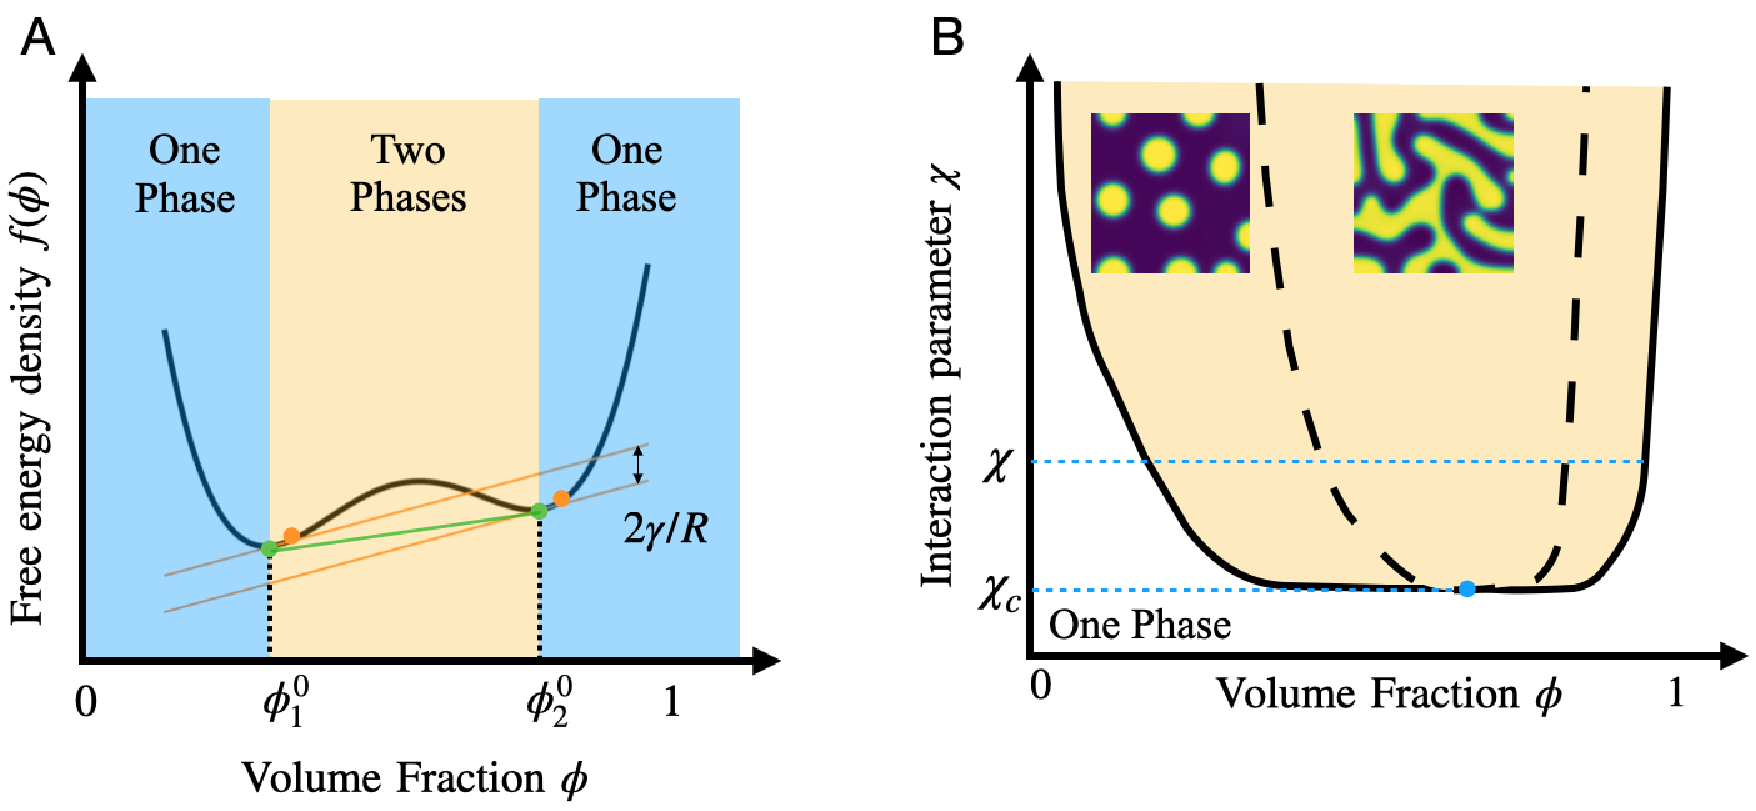
\includegraphics[scale=0.52]{MainContent/Figures/free_energy.pdf}
\caption{\textbf{Schematics of the free energy density for a binary system and the corresponding phase diagram.}
(A) shows schematics for an asymmetric free energy density for $\chi > \chi_c$ as a function of volume fraction $\phi$.
Phase separation is possible only when the average volume fraction lies between $\phi^0_1,~\phi^0_2$.
In the thermodynamic limit, the equilibrium volume fractions $[\phi^0_1,~\phi^0_2]$ (green dots) satisfying \Eqsref{eqn:constraint_1} are the minima of the free energy density.
For the case when phase separation occurs and a droplet of radius $R$ forms, the equilibrium volume fractions (orange dots) shift slightly to the right and the tangents at the equilibrium volume fractions differ in height by a value given by the \textit{Laplace pressure}.
(B) Phase diagram for the system for different interaction parameters $\chi$ as a function of the volume fraction $\phi$.
Below the critical interaction parameter $\chi < \chi_c$, only one phase (the homogeneous state) exists.
The phase boundary (thick black line); also known as the binodal, separates this region from regions where phase separation is possible.  
For $\chi > \chi_c$, lie two different regimes, namely the nucleation and growth regimes and the spinodal decomposition regime.
Between the binodal and the spinodal (dashed black line), we have the nucleation and growth regime which suppresses any infinitesimal perturbations.
For low $\phi$, sufficiently finite perturbations are required for droplets (in yellow) to nucleate and grow in size in the dilute phase (in blue) and for high value of $\phi$, droplets and dilute phase simply swap places.
Note that this regime is possible for low and high values of $\phi$, and for intermediate $\phi$ (spinodal decomposition regime), infinitesimal perturbations grow and system phase separates into bi-continuous structures.
The intersection of the binodal and the spinodal is $\chi_c$ (blue dot), which in the case of equal molecular volumes for $A,~B$ is $\chi_c = 2$ and occurs at $\phi = 0.5$; see Ref. \cite{Review2019}. 
}
\label{fig:free_energy}
\end{figure}

\section{Two-phase co-existence with an interface}

In a system with two phases separated by an interface, the free energy density will have contributions from the interfacial region in terms of the volume fraction $\phi$ and it's spatial gradients $\boldsymbol{\nabla} \phi$; see Refs. \cite{Review2019,Cahn1958}.
After integrating this free energy density with the interfacial contributions over the volume $V$ of the system, the total free energy density of the system reads as a functional of $\phi$; see Refs. \cite{Review2019,Cahn1958}, as:

\begin{equation}
\label{eqn:total_free_energy_FL}
\begin{split}
F[\phi] &= \frac{1}{\nu} \int \mathrm{d}V~ \bigg{[} \frac{\kappa}{2 \nu} |\boldsymbol{\nabla} \phi|^2 + \frac{z}{2} \left[ e_{AA} \phi +  e_{BB} (1 - \phi)\right] \\ & +  k_b T \left[ \phi \ln(\phi) + (1 - \phi) \ln (1 - \phi) + \chi \phi (1 - \phi) \right] \bigg{]}
\end{split}
\end{equation}

However, \Eqref{eqn:total_free_energy_FL} contains logarithmic terms, which can be avoided by considering a simpler form of the total free energy, namely the \textit{Ginzburg-Landau} free energy; see Ref. \cite{Review2019}, which reads as:

\begin{equation}
\label{eqn:total_free_energy_GL}
    F[\phi] = \int \left( f_{\mathrm{GL}}(\phi) +  \frac{\kappa}{2} |\boldsymbol{\nabla} \phi|^2 \right) \mathrm{d}V,
\end{equation}
where $f_{\mathrm{GL}}(\phi)$ is the \textit{Ginzburg-Landau} free energy density and $\kappa > 0$ is a parameter related to the interfacial tension; see Refs. \cite{Zwicker2015,Review2019}.
An important point has to be made from \Eqref{eqn:total_free_energy_GL}: the contribution of the the gradient energy term $\kappa|\boldsymbol{\nabla} \phi|^2 / 2$ gets lower when interface width gets wider or more diffuse; see Ref. \cite{Cahn1958}.
But this reduction in energy can only be compensated by increasing material at the interface, thereby increasing $f_{\mathrm{GL}}(\phi)$.
The gradient term hence penalizes strong variations in the volume fractions across the interface.

The reason we prefer using the \textit{Ginzburg-Landau} free energy density $f_{\mathrm{GL}}(\phi)$ from \Eqref{eqn:total_free_energy_GL} instead of the free energy density given by \Eqref{eqn:flory_huggins} or \Eqref{eqn:free_energy_formulationB} is that $f_{\mathrm{GL}}$ qualitatively captures the relevant features of phase separation such as the existence of two minima, concave and convex regions and a term which represents the interaction term favouring phase separation.
Additionally, the \textit{Ginzburg-Landau} free energy density also has a similar stability criterion and regimes of phase separation; see \figref{fig:free_energy}, as the free energy density given by \Eqref{eqn:flory_huggins} (or \Eqref{eqn:free_energy_formulationB}); see Appendix \ref{sec:phasesep}.

Henceforth, from this point onwards in the thesis, we consider the \textit{Ginzburg-Landau} free energy density which has a simple polynomial form and reads as:
\begin{equation}\label{eqn:free_energy}
    f_{\mathrm{GL}}(\phi) = f(\phi) = \frac{b}{2}(\phi - \phi^{0}_\mathrm{out})^2(\phi - \phi^{0}_\mathrm{in})^2,
\end{equation}
where the minima $\phi^{0}_\mathrm{in}$ and $\phi^{0}_\mathrm{out}$ are the equilibrium concentrations in a thermodynamically large system and $b$ denotes the energy scale.
Typically, we assume that in the thermodynamic limit, $\phi^{0}_\mathrm{in}$ will be a phase rich in droplet material A and $\phi^{0}_\mathrm{out}$ will be a phase rich in dilute phase material B, and hence the notation [in/out].

To summarize, for a system of two phases with an interface, we can calculate the total free energy from \Eqref{eqn:total_free_energy_GL}.
However, we can simply separate the energy contribution of the bulk phases and the energy contribution from the interface; see Ref. \cite{Review2019}, and arrive at explicit relations for the interface width $w$ and surface tension $\gamma$, which we define and discuss in the next section. 

\section{Interface width and surface tension}

In a system of two phases with an interface, we can approximately separate the energy contribution of the bulk phases and the energy contribution from the interface as:
\begin{equation*}
    F \approx V_1 f(\phi_1) + V_2 f(\phi_2) + F_\mathrm{interface},
\end{equation*}
where $F_\mathrm{interface}$ is the free energy associated with the interface.
In a thermodynamically large system, we can assume that if the interface is sharp, i.e. the variation in the phases occurs on a length-scale which is small as compared to the system size, it can be approximated as a surface.
Hence, we can approximate $F_\mathrm{interface} \approx S \gamma$, where $S$ is the surface area of the interface and $\gamma$ is the free energy per surface area of the interface, also known as \textit{surface tension}.

As the gradient term $\kappa|\boldsymbol{\nabla} \phi|^2 / 2$ in \Eqref{eqn:total_free_energy_GL} penalizes strong variations; see Ref. \cite{Cahn1958} in the volume fractions across the phases, it will be the dominant term in \Eqref{eqn:total_free_energy_GL} near the interface.
This forces the system to have a finite interface width $w$, which can be calculated  by considering a flat interface at position $x= 0$ in a one dimensional thermodynamically large system.
The equilibrium volume fractions far from the interface read as $\phi|_{x \rightarrow -\infty} = \phi^0_\mathrm{in}$ and $\phi|_{x \rightarrow \infty} = \phi^0_\mathrm{out}$.
The total free energy of the system given by \Eqref{eqn:total_free_energy_GL} is minimized when the volume fraction profile across the phases reads as:
\begin{equation*}
    \phi(x) = \frac{\phi^0_\mathrm{in} + \phi^0_\mathrm{out}}{2} + \frac{\phi^0_\mathrm{in} - \phi^0_\mathrm{out}}{2} \, \tanh{\left(\frac{x}{w} \right)},
\end{equation*}
where $w$ is the interface width given by $w = 2 \sqrt{\kappa/b}$ in our case; see Refs. \cite{Zwicker2015,Review2019}.

We can also calculate the surface tension $\gamma$ by considering a flat interface of area $S$ at position $x = 0$ in a thermodynamically large system.
The surface tension can now be defined with the contributions from the interfacial region as:
\begin{equation*}
    \gamma = \int_{-\infty}^{+ \infty} \left ( F[\phi(x)] - \frac{F[\phi^0_\mathrm{in}] + F[\phi^0_\mathrm{out}]}{2} \right)~\mathrm{d}x.
\end{equation*}
which in our case reads as $\gamma = (1/6) \sqrt{b/ \kappa}$; see Refs. \cite{Zwicker2015,Review2019}.

Having calculated explicit expressions for surface tension $\gamma$ and interface width $w$, we now assume that we have two phases separated by an interface.
Furthermore, the phase consisting of molecules of $A$ typically forms a droplet of radius $R$ embedded in the phase rich with molecules of $B$ (dilute phase) and we next discuss the effects of surface tension on such finite sized phase separated droplets.

\section{Effect of surface tension on droplets}

Consider a spherical droplet of radius $R \gg w$ formed by liquid-liquid phase separation from the dilute phase in a system of volume $V$. 
Let $\phiEqIn$ and $\phiEqOut$ denote the equilibrium volume fractions of droplet material $A$ inside and outside the droplet respectively.
The total free energy of such a system can simply be approximated by the sum of the contributions from the droplet and the dilute phase as:
\begin{equation}\label{eqn:constraint_3}
    F \approx V_d\,f(\phiIn) + (V - V_d)\,f(\phiOut) + S\,\gamma,
\end{equation}
where $V_d = (4/3) \pi R^3$ is the volume of the droplet, $S = 4 \pi R^2$ is the surface area of the droplet and $\gamma$ is the interfacial surface tension. 
From mass conservation, the total amount of droplet material must be conserved.
Hence,
\begin{equation}\label{eqn:constraint_4}
    V\,\overline{\phi} = V_d\,\phiIn + (V - V_d)\,\phiOut,
\end{equation}
Similar to the treatment for \Eqsref{eqn:constraint_1}, we again minimize the total free energy from \Eqref{eqn:constraint_3} by taking the derivatives with respect to $\phiIn, V_d$ to arrive at the necessary conditions as:

\begin{subequations}
\label{eqn:constraint_5}
\begin{align}
    f'(\phiIn) - f'(\phiOut) &= 0 \mathrm{~and~}
    \\[10pt]
    f(\phiIn) - f(\phiOut) - f'(\phiOut)(\phiIn - \phiOut) + \frac{2 \gamma}{R} &= 0.
\end{align}
\end{subequations}
Similar to \Eqsref{eqn:constraint_1}, the first condition implies that the chemical potential are equal inside and outside the droplet.
Similarly, the second condition states that the difference in the pressure inside and outside the droplet is a term which is directly proportional to a the surface tension $\gamma$ and inversely proportional to the droplet radius $R$, a term also known as \textit{Laplace pressure}; see Ref. \cite{Review2019}.

The equilibrium volume fractions $\phiEqIn,~\phiEqOut$ (orange dots in \figref{fig:free_energy}A) satisfying \Eqsref{eqn:constraint_5} can again be determined from \textit{Maxwell's construction} as follows:
We construct two tangent lines (orange lines in \figref{fig:free_energy}A), which differ in their height by a value of $2 \gamma / R$, and find the points of intersection of these tangents with the free energy density $f(\phi)$.
Note that contrary to the situation of thermodynamic limit, $\phiEqIn,~\phiEqOut$ no longer correspond to the minima of $f(\phi)$, but now get shifted slightly to the right (orange dots in \figref{fig:free_energy}A), as a result of a finite \textit{Laplace pressure}.
In the limit of the droplet radius $R \rightarrow \infty$, we recover $\phiEqIn,~\phiEqOut$ as the minima of $f(\phi)$ (green dots in \figref{fig:free_energy}A). 

We can also explicitly derive the expressions for the equilibrium volume fractions inside and outside the droplet $\phiEqIn,~\phiEqOut$.
From \Eqsref{eqn:constraint_5}, we can expand them as $\phiEqIn = \phi^0_\mathrm{in} + \delta \phiIn$ and $\phiEqOut = \phi^0_\mathrm{out} + \delta \phiOut$ to linear order in $\delta \phiIn$ and $\delta \phiOut$, where $\phi^0_\mathrm{in}$ and $\phi^0_\mathrm{out}$ are the equilibrium volume fractions in the thermodynamic limit; see Ref. \cite{Review2019}.
We then obtain
\begin{subequations}
\label{eqn:delta_phi_in_out}
\begin{align}
    \delta \phiOut &= \frac{2 \gamma}{[\phi^{0}_\mathrm{in} - \phi^{0}_\mathrm{out}] f''(\phi^{0}_\mathrm{out}) R} \mathrm{~and~}
    \\[10pt]
    \delta \phiIn &= \frac{f''(\phi^{0}_\mathrm{out})}{f''(\phi^{0}_\mathrm{in})} \delta \phiOut.
\end{align}
\end{subequations}
Note that $\delta \phiIn,~\delta \phiOut$ are positive, implying that surface tension slightly elevates the equilibrium volume fractions inside and outside the droplets from the basal values $\phi^{0}_\mathrm{in},~\phi^{0}_\mathrm{out}$ (which are the equilibrium volume fractions in the droplet phase and the dilute phase in the thermodynamic limit).
This effect is also inversely proportional to the droplet radius $R$, implying larger droplets are less affected than small droplets. 
This has a consequence when we discuss \textit{Ostwald-Ripening} in detail in a later section. 

To better see the effect of surface tension $\gamma$ on the droplets, we re-write \Eqsref{eqn:delta_phi_in_out} as:
\begin{subequations}
\label{eqn:GibbsThompsonRelations}
\begin{align}
    \phiEq_\mathrm{in} &= \phi^{0}_\mathrm{in} \left (1 + \frac{l_{\gamma, \mathrm{in}}}{R} \right )
    \mathrm{~and~}
    \\[10pt]
    \phiEq_\mathrm{out} &= \phi^{0}_\mathrm{out} \left ( 1 + \frac{l_{\gamma, \mathrm{out}}}{R}\right )
    \;,
\end{align}
\end{subequations}
where $l_{\gamma, \mathrm{out}}$ and $l_{\gamma, \mathrm{in}}$ are capillary lengths given by:

\begin{subequations}
\label{eqn:l_gamma}
\begin{align}
    l_{\gamma, \mathrm{in}} &= (\kappa/b)^{1/2} /[3 \phi^{0}_\mathrm{in} \left(\phi^{0}_\mathrm{in} - \phi^{0}_\mathrm{out}\right)^{3}] \nonumber 
    \mathrm{~and~}
    \\[10pt]
    l_{\gamma, \mathrm{out}} &= (\kappa/b)^{1/2} /[3 \phi^{0}_\mathrm{out} \left(\phi^{0}_\mathrm{in} - \phi^{0}_\mathrm{out}\right)^{3}], \nonumber
\end{align}
\end{subequations}
in the case of the free energy density given by \Eqref{eqn:free_energy} discussed in this thesis.
Since we consider strong phase separation $(\phi^{0}_\mathrm{in} \gg \phi^{0}_\mathrm{out})$, a consequence of \Eqsref{eqn:l_gamma} is $l_{\gamma, \mathrm{out}} \gg l_{\gamma, \mathrm{in}}$, leading to approximating the volume fraction inside the droplet as $\phiIn \approx \phi^{0}_\mathrm{in}$.
Thus, the curvature of the droplets mostly only affects $\phiOut$.
Hence, we finally arrive at the effects of surface tension on the basal values $\phi^{0}_\mathrm{in},~\phi^{0}_\mathrm{out}$, for a droplet of radius $R$.

To summarize, if we start with a homogeneous phase in the spinodal regime (see \figref{fig:free_energy}B), the system is unstable, so any perturbations in the system grow and we end up with two bulk phases; see Appendix \ref{sec:phasesep}. 
However, if we start with a homogeneous phase in the nucleation and growth regime, droplets nucleate for sufficiently high perturbations, and grow by taking up material from the dilute phase.

Having introduced the various phases possible from the free energy density given by \Eqref{eqn:free_energy}, we next introduce the dynamical equations for such phase-separating systems.

% As we are primarily interested in modelling the dynamics of phase separated droplets, in this thesis we will focus solely on the nucleation and growth regime and consider that perturbations are sufficiently finite and droplets form.

\section{Continuous model of phase separation for passive systems}

The dynamics of the system follow from the continuity equation:
\begin{equation*}
    \frac{\partial \phi}{\partial t} + {\boldsymbol{\nabla}} \cdot \vec{j} = 0,
\end{equation*} 
where $\vec{j}$ denotes diffusive fluxes which are driven by gradients in chemical potential $\mu$; see Ref. \cite{Review2019}, which in our case of the free energy density (\Eqref{eqn:free_energy}) becomes:
\begin{equation}
\label{eqn:chemical_potential}
    \mu = \nu \frac{\delta F}{\delta \phi} = b (\phi^{0}_\mathrm{in} - \phi) (\phi^{0}_\mathrm{out} - \phi) (2\phi - \phi^{0}_\mathrm{in} - \phi^{0}_\mathrm{out}) - \kappa \nabla^2 \phi,
\end{equation}
where $\nu$ is the molecular volume of the droplet material.
Linear non-equilibrium thermodynamics implies that the fluxes are proportional to gradients in the chemical potential; see Ref. \cite{Review2019}, which reads as:
\begin{equation*}
    \vec{j} = -\Lambda(\phi) {\boldsymbol{\nabla}}\mu,
\end{equation*}
where $\Lambda(\phi)$ is a positive mobility; see Ref. \cite{GrootBook}.
Hence, the resulting equation takes the form:
\begin{equation} \label{eqn:CHPassive}
    \frac{\partial \phi}{\partial t} = {\boldsymbol{\nabla}} \cdot [\Lambda(\phi) {\boldsymbol{\nabla}} \mu],
\end{equation}
which we will refer to hence-forth in this thesis as the \textit{Continuous model} of phase separation.
\Eqref{eqn:CHPassive} is traditionally also known as the \textit{Cahn-Hilliard} equation; see Refs. \cite{Cahn1958,CahnHilliardEq}, which describes passive phase separation.
In this thesis, we will refer to \Eqref{eqn:CHPassive} and it's counterpart with chemical reactions \Eqref{eqn:CHActive} as the continuous model. 
In particular, two bulk phases with composition $\phi^{0}_\mathrm{in}$ and $\phi^{0}_\mathrm{out}$ typically emerge, which are separated by a typically thin interface of width $w = 2 \sqrt{\kappa/b}$ and surface tension $\gamma = (1/6) \sqrt{b/ \kappa}$.

Consider now a system of droplets formed from sufficiently finite perturbations inside the nucleation and growth regime; see Appendix \ref{sec:phasesep}.
Droplets with smaller radius will have a larger Laplace pressure $(\propto R^{-1})$ and droplets with higher radius will consequently have a smaller Laplace pressure. 
This difference causes a gradient of the chemical potential between the droplets and thus material flows from the smaller to the larger droplets, a process known as \textit{Ostwald-Ripening}; see Ref. \cite{Review2019}.
Eventually, only one droplet remains, and we will elaborate more on this process in Chapter \ref{chap:Chapter_5}.
Naturally, such a coarsening is not favourable for biomolecular condensates, as their size and location needs to be controlled by the cell in order to perform various biomolecular functions.
One such way of suppressing this coarsening behaviour is introduction of chemical reactions and make the system \textit{active}; see Refs. \cite{Zwicker2015,Review2019,Glotzer1995}, which we will discuss in the following section.

\section{Continuous model of passive phase separation with chemical reactions}

We now consider simple chemical reactions which convert the droplet material $A$ into dilute phase material $B$ and vice versa, in which case the individual number of molecules of $A,B$ are no longer conserved, but their sum is.
We assume that the chemical reactions are typically local and can be often described by rate laws that depend on the composition.

In addition, we consider chemical reaction schemes which do not obey detailed balance because in a reaction scheme obeying detailed balance, $A$ and $B$ can convert into each other and the volume fractions $\phiIn, \phiOut$ will relax into states where the total free energy is minimized for a given average volume fraction $\overline{\phi} = \frac{\int_V \phi ~ \mathrm{d}V}{V}$.
This state is usually the homogeneous state consisting of no droplets and hence broken detailed balance is necessary; see Refs. \cite{Zwicker2015,Review2019}.

However, breaking of detailed balance is partly inspired from Biology as well.
For example, $A, B$ can represent two states of a protein with their conversion facilitated by phosphorylation dephosphorylation reactions, when the energy source is adenosine triphosphate molecules; see Ref. \cite{AlbertsBook2003}.
Aguilera-Gomez et al. \cite{Aguilera_Gomez2017} highlighted the general importance of MARylation in the formation and control of condensates in the \textit{Drosophila} oocyte.
Similarly, phosphorylation of NBDY (which is an intrinsically disordered protein) has been shown by Na et al. \cite{Na2021} to be linked with the stability of P-bodies.
Similarly, Saurabh et al. \cite{Saurabh2022} showed in vivo that ATP depletion promotes phase separation in eukaryotic cells, also see Ref. \cite{Pattanayak2020}.

Strong chemical reactions can actually destroy droplets and/or lead to droplet splitting; see Ref. \cite{Zwicker_nature_2016} and they might also lead to more complicated patterns; see Refs. \cite{Glotzer1995,Christensen1996}, which go beyond the scope of this thesis.
Hence, in this thesis, we consider situations in which detailed balance is broken, subsequently leading to novel non-equilibrium effects in the system.
For example, Zwicker et al. \cite{Zwicker2015,Zwicker2014} showed that \textit{Ostwald-Ripening} is shown to be suppressed when simple first order chemical reactions are present between the droplet and the dilute phase material and multiple droplets can co-exist.
Influence of chemical gradients on phase separation has been studied by Weber et al. \cite{Weber2017} and revealed a physical mechanism for arresting droplet ripening.

In this thesis, we focus on situations of weak reaction rates and hence, chemical reactions introduce only a local sink/source term $s(\phi)$ in the continuity equation; see Refs. \cite{Zwicker2015,Review2019}, as:
\begin{equation*}
    \frac{\partial \phi}{\partial t} + {\boldsymbol{\nabla}} \cdot \vec{j} = s(\phi),
\end{equation*}
and the resulting dynamical equation then takes the form:
\begin{equation} \label{eqn:CHActive}
   \frac{\partial \phi}{\partial t} = {\boldsymbol{\nabla}} \cdot [\Lambda(\phi) {\boldsymbol{\nabla}} \mu] + s(\phi).
\end{equation}
and we arrive at the dynamics of the system when local chemical reactions are present.
Note that \Eqref{eqn:CHActive} is a fourth-order, non-linear partial differential equation requiring two boundary conditions for $\phi, ~\mu$.
We here focus on the typical choice of no-flux conditions ($\vec{n} \cdot {\boldsymbol{\nabla}} \mu = 0$) and ($\vec{n} \cdot {\boldsymbol{\nabla}} \phi = 0$), implying that dilute phase and droplet material interact identically with the system's boundaries, whose normal vector is denoted as $\vec{n}$.

\section{Thin interface approximation of the continuous model}

We now arrive at an important junction in this thesis. 
Till now, we have presented basic principles of phase separation for an incompressible binary fluid system and arrived at the effects of chemical reactions on the dynamics of phase separation.

Our aim in this thesis is to numerically simulate phase separation phenomena, in particular, the dynamics of phase separated droplets.
We hence restrict ourselves to the nucleation and growth regimes of phase separation, and do not consider the spinodal growth regime; see \figref{fig:free_energy}B.
Furthermore, we assume that owing to sufficiently finite perturbations, well defined droplets with typical radius $(R \gg w)$ have been phase separated from the dilute phase, and we do not consider any nucleation events.
Simply put, we assume that droplets bigger than the interface width $w$ have been formed as a result of sufficiently finite perturbations in the nucleation and growth regime, whose dynamics we are interested in simulating.

The dynamics of such a system with droplets phase separated from the dilute phase is adequately described by \Eqref{eqn:CHActive}.
But beyond the linear regime (i.e. close to $\phi^0_\mathrm{in}, ~\phi^0_\mathrm{out}$ from \Eqref{eqn:free_energy}), \Eqref{eqn:CHActive} is difficult to solve analytically, as it is non-linear and contains fourth order spatial derivatives.
The continuous model, given by \Eqref{eqn:CHActive}, can also be prohibitively costly to simulate due to multiple reasons:
\begin{enumerate}
    \item The interface needs to be spatially resolved, implying that the spatial discretization of the system should be smaller than the typically small interface width $w$.
    Since we typically consider dilute system of many droplets, simulations are computationally expensive because regions far away from the droplet interfaces typically exhibit very low variation in the volume fraction $\phi$ as seen from Fig. \ref{fig:schematics_CH}.
    
    \item \Eqref{eqn:CHActive} contains fourth order spatial derivatives, which limits the time steps to extremely small values.
    
    \item Interesting and relevant dynamics usually takes place on very long time scales, for instance: during \textit{Ostwald-Ripening}, the length scales in the system evolve as $t^{\,1/3}$ following the Lifshitz-Slyozov-Wagner scaling laws; see Refs. \cite{Lifshitz,Wagner}.
    This typically requires long simulations to capture the relevant behaviour.
\end{enumerate}
Owing to these limitations, simulations of phase separated droplets become extremely computationally expensive.
From typical simulations of phase separated droplets using the continuous model; see Fig. \ref{fig:schematics_CH}, we make certain observations which can enable us to simulate such system of droplets faster and efficiently.

\clearpage

\begin{figure}[tb]
\centering
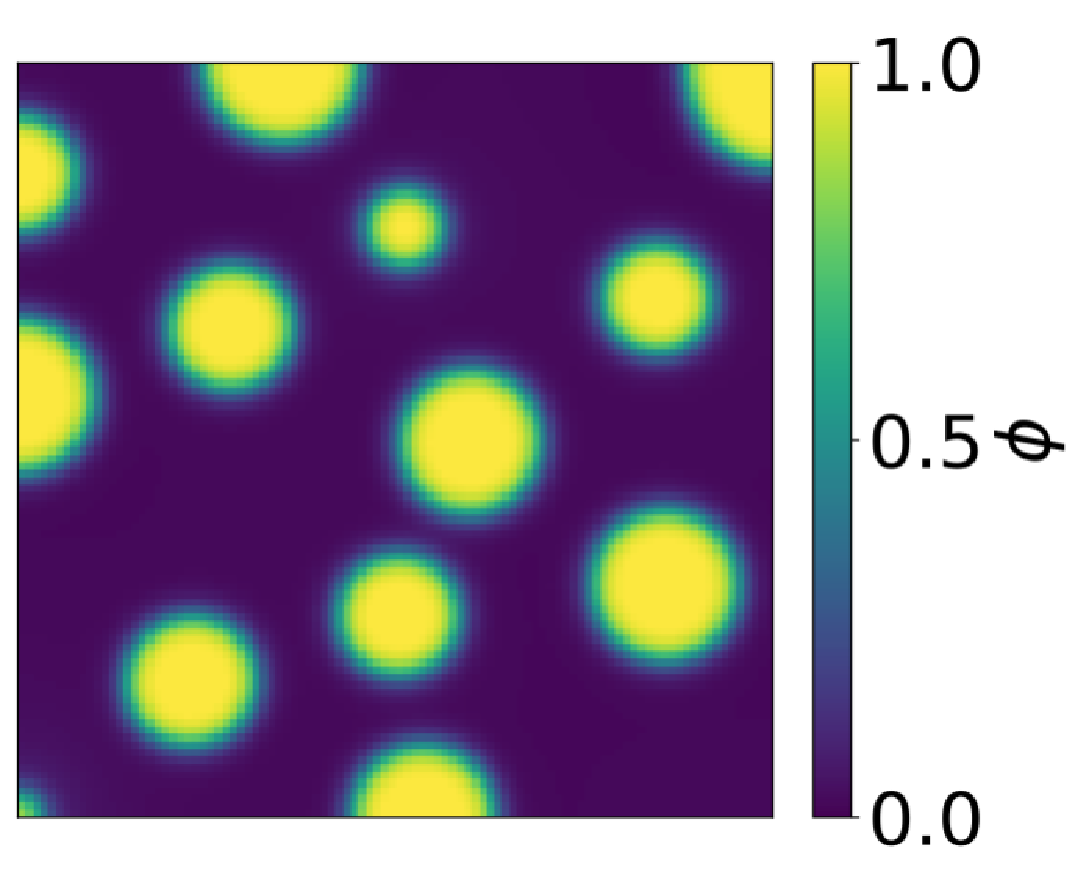
\includegraphics[scale=0.35]{MainContent/Figures/Simulation_CH_Passive.pdf}
\caption{\textbf{Typical simulation state for the continuous model.}
Figure shows a typical state for simulations of the continuous model (\Eqref{eqn:CHActive}, $s(\phi) = 0$) in the nucleation and growth regime depicting the volume fraction field $\phi$.
Phase separated droplets (yellow, with $\phiIn \approx \phi^{(0)}_\mathrm{in}$) are round and variation of $\phiIn,~\phiOut$ in the droplets and dilute phase (blue, with $\phiOut \approx \phi^{(0)}_\mathrm{out}$) itself is low.
The basal values are chosen as $\phi^{(0)}_\mathrm{out} = 0$ and $\phi^{(0)}_\mathrm{in} = 1$ from \Eqref{eqn:free_energy}.
% The continuous model (\Eqref{eqn:CHActive}, $s(\phi) = 0$) uses a two dimensional Cartesian grid of discretization $0.5w$, $w = 2 \sqrt{\kappa / b}$, initial volume fraction $\phi(t=0)$ uniformly chosen from $[\phi = 0.2,0.3]$, $s=0$, $\Lambda = \textcolor{red}{???}$, $\phi^{(0)}_\mathrm{out} = 0$ and $\phi^{(0)}_\mathrm{in} = 1$.
}
\label{fig:schematics_CH}
\end{figure}

The observations we make are:
\begin{enumerate}
    \item Droplets are typically round due to surface tension effects, with the interface $w$ typically smaller than the droplet radius ($R \gg w$).
    Typically, the interfacial width $w$ varies from $10-100\,\mathrm{nm}$; see Ref. \cite{safran_2003}, and is often a small quantity compared to the typical length-scales in the system. 
    
    \item Strong phase separation exists between the droplet and the dilute phases, i.e. $\phi^{0}_\mathrm{in} \gg \phi^{0}_\mathrm{out}$; see \figref{fig:free_energy}A.

    \item Far away from the droplets, spatial variation in the volume fractions is low inside the droplets and the dilute phase itself.

\end{enumerate}
Since we have strong phase separation and low spatial variation of volume fractions inside the droplet phase and inside the dilute phase, we can linearize \Eqref{eqn:CHActive} around $\phi^{0}_\mathrm{in},~\phi^{0}_\mathrm{out}$ to obtain the reaction-diffusion equations which hold inside both the phases; see Ref. \cite{Review2019}, as:

\begin{equation}
\label{eqn:thin_interface_model}
   \frac{\partial \phi_\mathrm{in/out}}{\partial t}
    \approx D_\mathrm{in/out} \nabla^2 \phi_\mathrm{in/out} +
    s(\phi_\mathrm{in/out}),
\end{equation}
where $D_\mathrm{in/out} = \Lambda(\phi^0_\mathrm{in/out})\,b$ is the diffusivity inside the droplets and outside the droplets respectively.
\Eqsref{eqn:thin_interface_model} is known as the \textit{thin-interface approximation}; see Ref. \cite{Zwicker2015}, of the continuous model.

Thus, we arrive at a framework where \Eqsref{eqn:thin_interface_model} enable us to separately consider the volume fractions inside the droplets ($\phiIn$) and outside the droplets, i.e. inside the dilute phase ($\phiOut$).
We will discuss these reaction-diffusion equations for dynamics of droplets and the dilute phase in more detail, in the next chapter.
Note that the quantities $\kappa, w$ and $\Lambda$ act as the link between the continuous model given by \Eqref{eqn:CHActive} and the dynamics of the droplets and dilute phase from \Eqsref{eqn:thin_interface_model}, as $\kappa, w$ appear in \Eqsref{eqn:GibbsThompsonRelations} when evaluating the equilibrium volume fractions for the droplets.

Hence, for phase separated droplets, we have separated the dynamical equations for the droplets and the dilute phase; see \Eqsref{eqn:thin_interface_model}, from the continuous model given by \Eqsref{eqn:CHActive}.
Note that \Eqsref{eqn:thin_interface_model} contain only second order spatial derivatives and hence are potentially much faster to simulate than \Eqsref{eqn:CHActive}.
In the next chapter, we discuss on the procedure of formulating a numerical scheme using \Eqsref{eqn:thin_interface_model} to simulate the dynamics of the droplets and the background field.
Since we separately consider dynamics of the droplets and the dilute phase, the thin interface formulation essentially separates the droplets in the foreground from the dilute phase material in the background. 
Hence, we will call the dilute phase as background field in this thesis from this point on-wards. 

\section{Summary}

In this chapter, we presented the basic principles of Liquid-liquid phase separation for an incompressible binary fluid system using statistical mechanics and linear equilibrium thermodynamics. 
We started with a microscopic picture of phase separation by considering a molecule based lattice model, where we defined interactions between pairs of molecules and used the \textit{mean-field approximation}; see Ref. \cite{Review2019}, to determine the free energy density and internal energy of the system; see \Eqsref{eqn:free_energy_formulation} and the \textit{Flory-Huggins} interaction parameter $\chi$; see \Eqref{eqn:chi}.
We showed from \figref{fig:free_energy}, that for large values of the interaction parameter $\chi > \chi_c$, the free energy density contains both - a concave and a convex part, thus potentially lowering the total free energy and phase separating the homogeneous mixture into two phases. 
Consequently, for $\chi < \chi_c$, only homogeneous phases are possible and thus, no phase separation.

With an aim to arrive at the dynamical equations of phase separation, we first determined the equilibrium volume fractions of the two phases when they phase separated: a) In the thermodynamic limit without an interface, and b) With the inclusion of an interfacial term.
Since we wanted to simulate dynamics of phase separated droplets, we 
focused on the nucleation and growth regimes and assumed finite sized droplets have formed via sufficiently finite perturbations in the homogeneous state.
Taking advantage of the simple form of the \textit{Ginzburg-Landau} free energy density (\Eqref{eqn:free_energy}) over the free energy density given by \Eqref{eqn:flory_huggins}, we used it to derive the effects of interface width $w$ and surface tension $\gamma$ on the equilibrium volume fractions (\Eqsref{eqn:GibbsThompsonRelations}) for droplets and found that they are elevated from the basal values $\phi^0_\mathrm{in},~\phi^0_\mathrm{out}$; see \Eqref{eqn:free_energy}.

We then derived the dynamical equations for passive phase separation by considering that gradients in chemical potential $\mu$ drive the material fluxes and arrived at the traditional \textit{Cahn-Hilliard} equation describing passive phase separation, given by \Eqref{eqn:CHPassive}. 
Next, we took into account the effect of local and weak chemical reactions, which break detailed balance and lead to novel physics, on passive phase separation and arrived at the dynamical equation for the system in presence of chemical reactions given by \Eqref{eqn:CHActive}.

Finally, we showed the limitations and drawbacks in simulating the continuous model; given by \Eqref{eqn:CHActive}, for simulating the dynamics of phase separate droplets.
Based on valid assumptions, we then formulated an approximated analytical model; given by \Eqsref{eqn:thin_interface_model}, which described the separation of the dynamics of droplets and the dilute phase using simple reaction-diffusion equations.